\documentclass[12pt]{article}

\usepackage{amssymb, amsmath, amsfonts}
\usepackage{amsthm}
\usepackage{moreverb}
\usepackage{graphicx}
\usepackage{enumerate}
\usepackage{graphics}
\usepackage{listings}
\usepackage{color}
\usepackage{array}
\usepackage{float}
\usepackage{hyperref}
\usepackage{textcomp}
\usepackage{alltt}
\usepackage{mathtools}
\usepackage[T1]{fontenc}
\usepackage{fullpage}
\usepackage{tikz}
\usepackage[utf8]{inputenc}
\newcommand{\suchthat}{\, \mid \,}
\usepackage{fancyvrb}
%\allowdisplaybreaks
\def\arraystretch{1.7}%  1 is the default, change whatever you need

\definecolor{codegreen}{rgb}{0,0.6,0}
\definecolor{codegray}{rgb}{0.5,0.5,0.5}
\definecolor{codepurple}{rgb}{0.58,0,0.82}
\definecolor{backcolour}{rgb}{0.95,0.95,0.92}
 
\lstdefinestyle{mystyle}{
    backgroundcolor=\color{backcolour},   
    commentstyle=\color{codegreen},
    keywordstyle=\color{magenta},
    numberstyle=\tiny\color{codegray},
    stringstyle=\color{codepurple},
    basicstyle=\footnotesize,
    breakatwhitespace=false,         
    breaklines=true,                 
    captionpos=b,                    
    keepspaces=true,                 
    numbers=left,                    
    numbersep=5pt,                  
    showspaces=false,                
    showstringspaces=false,
    showtabs=false,                  
    tabsize=2
}
 
\lstset{style=mystyle}

\begin{document}

{\bf MATH 481A \hfill Numerical Analysis \ \ \ \ \ \hfill Spring 2015}

\title{\bf Lab \# 1 Solutions}
\author{\bf Sam Fleischer}
\date{\bf Tues. Mar. 3, 2015}

{\let\newpage\relax\maketitle}
\maketitle
\tableofcontents
\pagebreak

\section*{Problem 1}
\addcontentsline{toc}{section}{Problem 1}
{\it Write a function named {\tt DivDiffs} that computes the table of divided differences of
the data $(x_0, y_0)$, $(x_1, y_1)$, $\dots$, $(x_n, y_n)$.  The function should take as input two 1-d arrays of size $n$, and return a 2-d array of size $n \times (n + 1)$ whose first two columns hold the data and the rest of the columns the divided differences.  Copy and paste the function in your lab report.}\\

\noindent I re-wrote the function to take a single 1-d array of size $n$ and a function.  That way the function values (y values) can be calculated within the function.
\begin{lstlisting}[language=Python, caption=Divided Differences Function] 
def DivDiffs(x_data, function):
    n = len(x_data)
    DD = np.zeros([n,n+1])

    DD[:,0] = x_data
    DD[:,1] = function(x_data)
    for column in range(2,n+1):
        for row in range(0, n+1-column):
            num = DD[row + 1,column - 1] - DD[row,column - 1]
            denom = DD[row + column - 1,0] - DD[row,0]
            DD[row,column] = (num)/(denom)
    return DD
\end{lstlisting}


\section*{Problem 2}
\addcontentsline{toc}{section}{Problem 2}
{\it Write a function named {\tt InterpolantDD} that takes as input the table of divided differences returned by the function of problem 1 and a list of x-values (within the interval delimited by the $x_i$'s) are returns the values computed by the interpolating polynomial that will result from those divided differences at those x-values.  Copy and paste the function in your lab report.}\\

\noindent I wrote a function called {\tt makePolynomial} that takes the divided difference table and returns the interpolated polynomial function.
\begin{lstlisting}[language=Python, caption=Forming Polynomials from Divided Difference Tables]
def makePolynomial(DD):
    def InterpolantDD(x):
        P = 0
        for i in xrange(0, len(DD[:,0])):
            term = 1
            for j in xrange(0, i):
                term *= (x - DD[0, j])
            term *= DD[0, i+1]
            P += term
    
        return P
    return InterpolantDD
\end{lstlisting}

\section*{Problem 3}
\addcontentsline{toc}{section}{Problem 3}
{\it Test the functions you wrote in {\bf Problem 1} and {\bf Problem 2} with the polynomials $p_3(x) = x(x-2)(x+2)$ and $p_5(x) = x(x-5)(x-2)(x+2)(x+5)$.  In each case:}
\begin{enumerate}[\ \ (a)\ \ ]
\item {\it Plot in the same window: $(i)$ the graph if the interplant, $P(x)$, vs. the list of $x$-values that of the given polynomial, and $(ii)$ the graph of the polynomial $p_j(x)$ vs x.}

\item {\it Plot the error, $|P(x) - p_j(x)|$, $j = 3, 5$},

\end{enumerate}
{\it Use four sample points for $p_3(x)$ six for $ p_5(x)$}\\

\noindent The following code was used to generate the graphs shown below.
\begin{lstlisting}[language=Python, caption=Problem 3]
def makePolyTest(*zeros):
    def poly_test(x):
        prod = 1
        for z in zeros:
            prod *= (x - z)
        return prod
    return poly_test

def error(f1, f2):
    def E(x):
        return abs(f1(x) - f2(x))
    return E

x_100           = np.linspace(-2.0,2.0,100)

x_4             = np.linspace(-2.0,2.0,4)
x_6             = np.linspace(-2.0,2.0,6)

poly_1          = makePolyTest(0, -2, 2)
poly_2          = makePolyTest(0, -2, 2, -5, 5)

DD_1            = DivDiffs(x_4,poly_1)
DD_2            = DivDiffs(x_6,poly_2)

interp_1        = makePolynomial(DD_1)
interp_2        = makePolynomial(DD_2)

error_1         = error(poly_1, interp_1)
error_2         = error(poly_2, interp_2)

p3_label        = r"$p_3(x)$"
p5_label        = r"$p_5(x)$"

p3_interp_label = r"$\overline{p_3}(x)$"
p5_interp_label = r"$\overline{p_5}(x)$"

p3_error_label  = r"$|p_3(x) - \overline{p_3}(x)|$"
p5_error_label  = r"$|p_5(x) - \overline{p_5}(x)|$"

plt.figure()
plt.plot(x_100, poly_1(x_100), "c", linewidth=2, label = p3_label)
plt.plot(x_100, interp_1(x_100), ".k", label = p3_interp_label)
plt.legend(loc=0)
plt.savefig("%s/figures/problem3_a.png" % DIRECTORY, format = 'png')
plt.close()

plt.figure()
plt.plot(x_100, poly_2(x_100), "c", linewidth=2., label = p5_label)
plt.plot(x_100, interp_2(x_100), ".k", label = p5_interp_label)
plt.legend(loc=0)
plt.savefig("%s/figures/problem3_b.png" % DIRECTORY, format = 'png')
plt.close()

plt.figure()
plt.plot(x_100, error_1(x_100), ".k", label = p3_error_label)
plt.legend(loc=0)
plt.savefig("%s/figures/problem3_a_error.png" % DIRECTORY, format = 'png')
plt.close()

plt.figure()
plt.plot(x_100, error_2(x_100), ".k", label = p5_error_label)
plt.legend(loc=0)
plt.savefig("%s/figures/problem3_b_error.png" % DIRECTORY, format = 'png')
plt.close()
\end{lstlisting}
\begin{enumerate}[\ \ (a)\ \ ]
\item In the following graphs, $p_3(x) = x(x-2)(x+2)$, $p_5(x) = x(x-2)(x+2)(x-5)(x+5)$, and $\overline{p_3}(x)$ and $\overline{p_5}(x)$ are the approximation of $p_3(x)$ and $p_5(x)$ obtained by creating the divided difference table with four and six data points, respectively.
\centerline{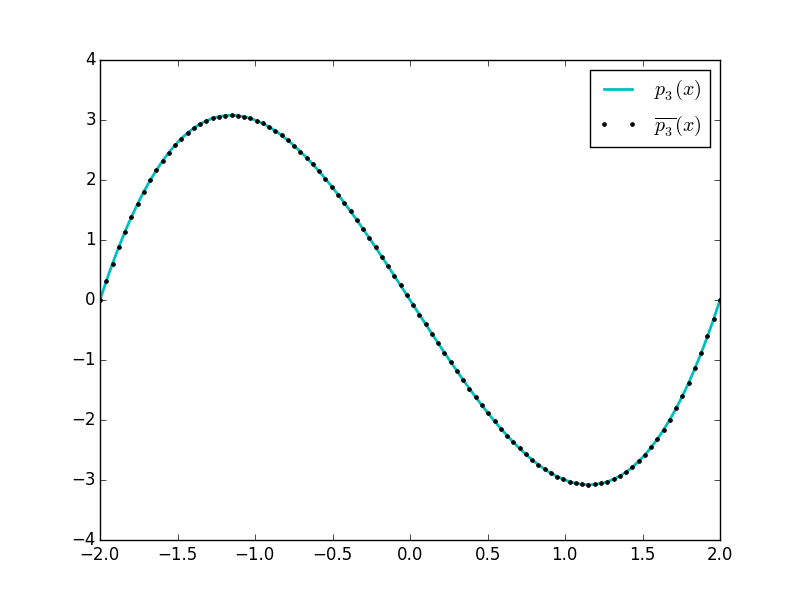
\includegraphics[scale=0.65]{figures/problem3_a.png}}\\
\centerline{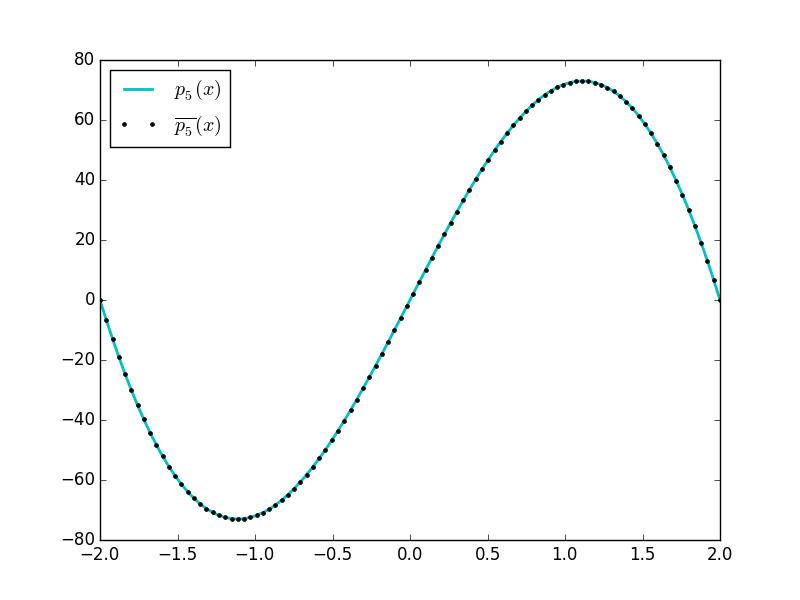
\includegraphics[scale=0.65]{figures/problem3_b.png}}
\item The following graphs show the error of approximations.\\
\centerline{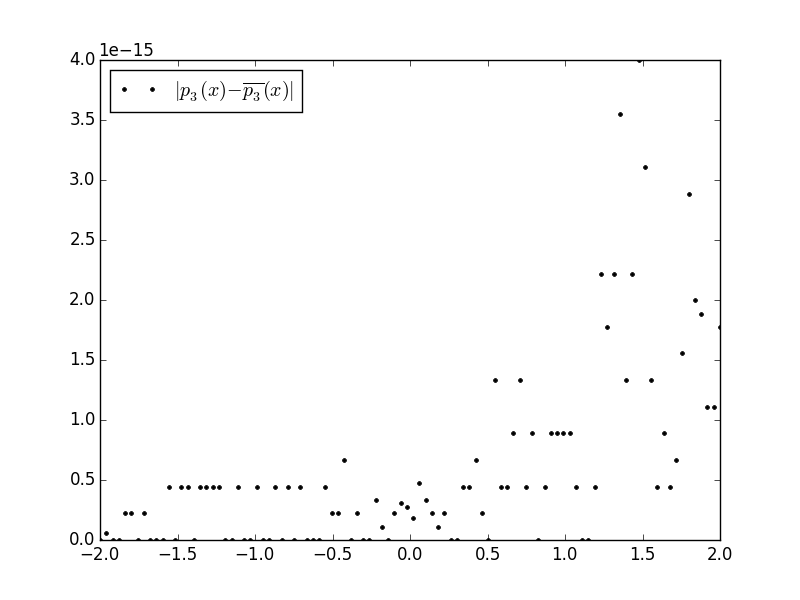
\includegraphics[scale=0.65]{figures/problem3_a_error.png}}\\
\centerline{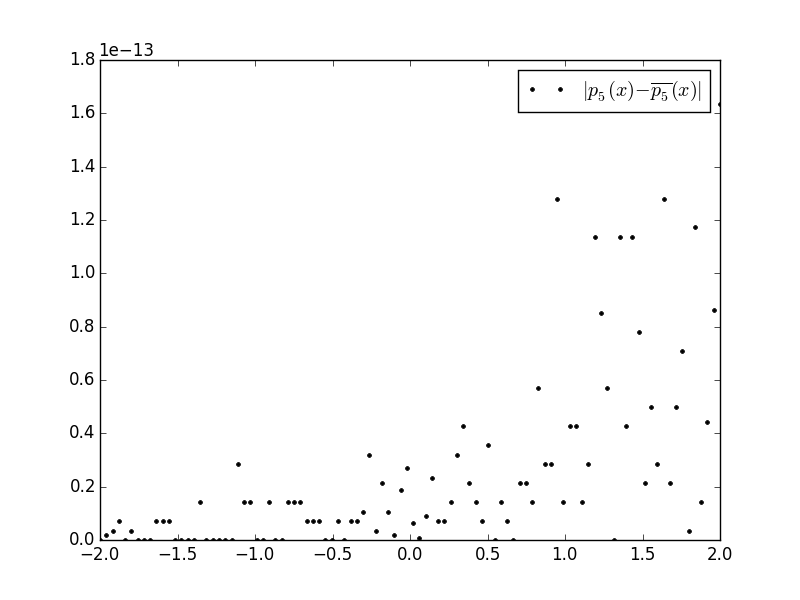
\includegraphics[scale=0.65]{figures/problem3_b_error.png}}\\
The error of the interpolated polynomials is small (on the order of $10^{-15}$ and $10^{-13}$, respectively) because the functions they are approximating are actually polynomials.  The theoretical error between $p_i(x)$ and $\overline{p_i}(x)$ is identically $0$ because an $n$\textsuperscript{th} degree polynomial is uniquely determined by $n+1$ data points.  The error we are seeing is computer truncation error.
\end{enumerate}

\section*{Problem 4}
\addcontentsline{toc}{section}{Problem 4}
{\it Consider the function}
\begin{align*}
f(x) = \frac{1}{1 + x^2}
\end{align*}
{\it Write a program that:}
\begin{enumerate}[\ \ (a)\ \ ]
\item {\it Selects $n$ equally spaced  $x$-values  in the interval $[-5, 5]$, and computes the corresponding  sample $y$-values using the definition of  $f(x)$.}
\item {\it Computes the divided differences of the  data generated in part {\rm (a)}.  For $n=5$, print the divided difference table in your lab report.}
\item {\it Selects 100 equally spaced $x$-values in the interval $[?5, 5]$, and computes the corresponding values $f(x)$ and $\overline{f}(x)$, the interpolating polynomial resulting from the divided differences of part {\rm (b)}.}
\item {\it Plots, in the same window, $f(x)$ vs. $x$ and $\overline{f}(x)$ vs. $x$.}
\item {\it Plots the error $|f(x) - \overline{f}(x)|$ vs. $x$.}
\item {\it Repeat parts {\rm (a)}-{\rm (e)} for $n = 10$, $20$, $30$, and include a table in your report with the maximum difference $|f(x) - \overline{f}(x)|$ for the 100 $x$-values you are evaluating both at.}
\item {\it Does the max error decrease as n increases? Is this a contradiction to Weierstrass Theorem?  Can you think of any way to decrease this error?}
\end{enumerate}

\noindent The following code was used to generate the graphs and table shown below:
\begin{lstlisting}[language=Python, caption=Problem 4]
def runge(x):
    return 1./(1.0 + (x**2))

for n in [5, 10, 20, 30]:
    x_n = np.linspace(-5.0, 5.0, n)
    
    DD_runge = DivDiffs(x_n, runge)
    interp_runge = makePolynomial(DD_runge)
    if n == 5:
        print DD_runge
    
    x_100     = np.linspace(-5.0, 5.0, 100)
    error_100 = abs(runge(x_100) - interp_runge(x_100))
    max_y     = max(error_100)
    max_index = list(error_100).index(max_y)
    max_x     = list(x_100)[max_index]
    
    runge_label        = "f(x)"
    runge_interp_label = "\overline{f_{%.02d}}(x)" % n
    runge_error_label  = "|%s - %s|" % (runge_label, runge_interp_label)
    max_error_label    = "max error: %.03f" % max_y
    
    file_name = "%s/figures/problem4_d_%.3dpoints.png" % (DIRECTORY, n)
    plt.figure()
    plt.plot(x_100, runge(x_100), "c", linewidth = 2., label = runge_label)
    plt.plot(x_100, interp_runge(x_100), ".k", label = runge_interp_label)
    plt.legend(loc=0)
    plt.savefig(file_name, format = 'png')
    plt.close()
    
    file_name = "%s/figures/problem4_e_%.3dpoints.png" % (DIRECTORY, n)
    plt.figure()
    plt.plot(x_100, error_100, ".k", label = runge_error_label)
    plt.plot(max_x, max_y, c="c", marker="^", label = max_error_label)
    plt.legend(loc=0)
    plt.savefig(file_name, format = 'png')
    plt.close()
\end{lstlisting}
The following graphs show $f(x)$ and its polynomial approximation $\overline{f_{05}}(x)$ for 5 equally spaced points, along with the error of the approximation.\\
\centerline{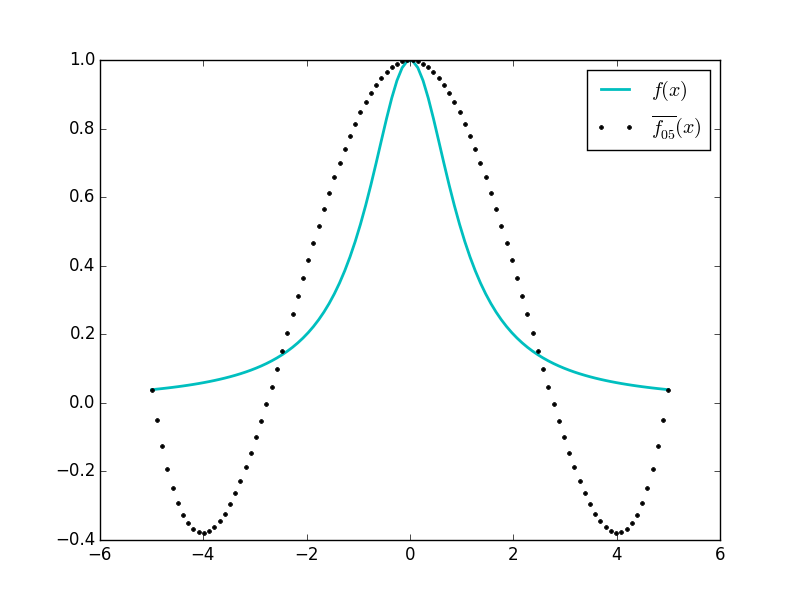
\includegraphics[scale=0.65]{figures/problem4_d_005points.png}}\\
\centerline{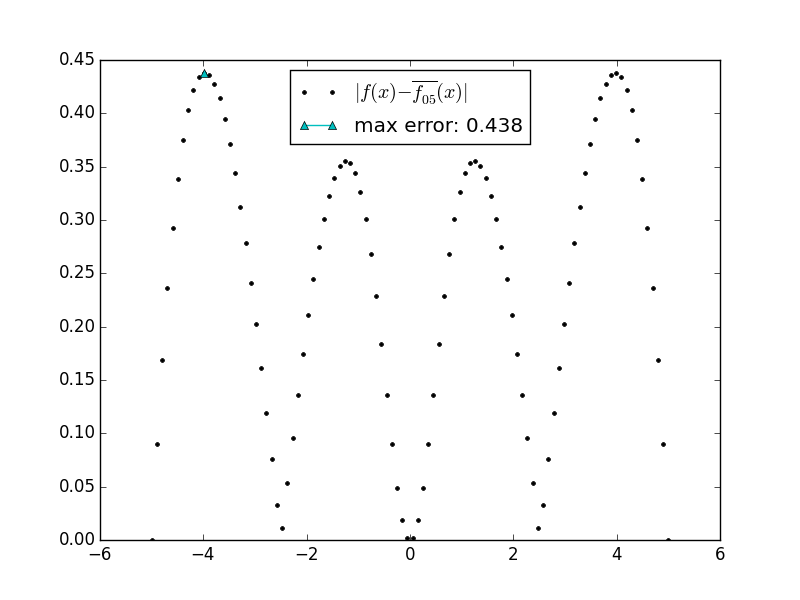
\includegraphics[scale=0.65]{figures/problem4_e_005points.png}}\\
The following graphs show $f(x)$ and its polynomial approximation $\overline{f_{10}}(x)$ for 10 equally spaced points, along with the error of the approximation.\\
\centerline{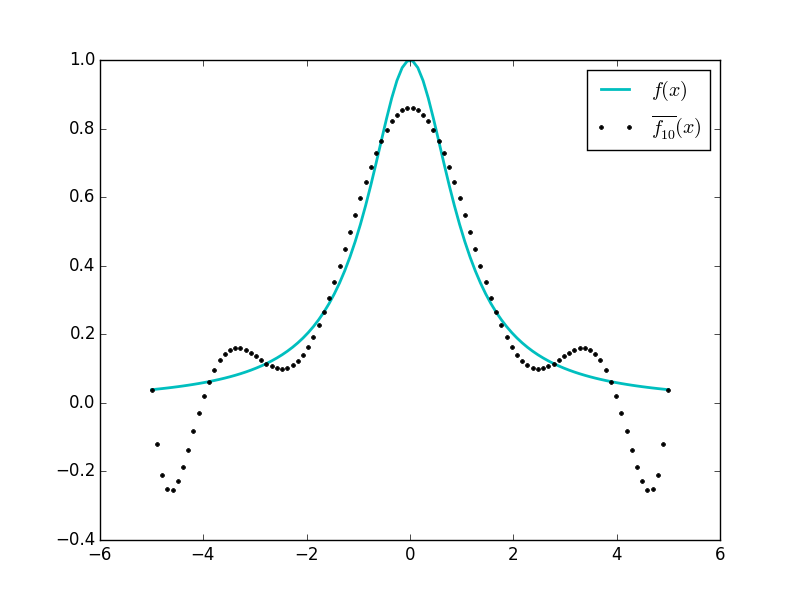
\includegraphics[scale=0.65]{figures/problem4_d_010points.png}}\\
\centerline{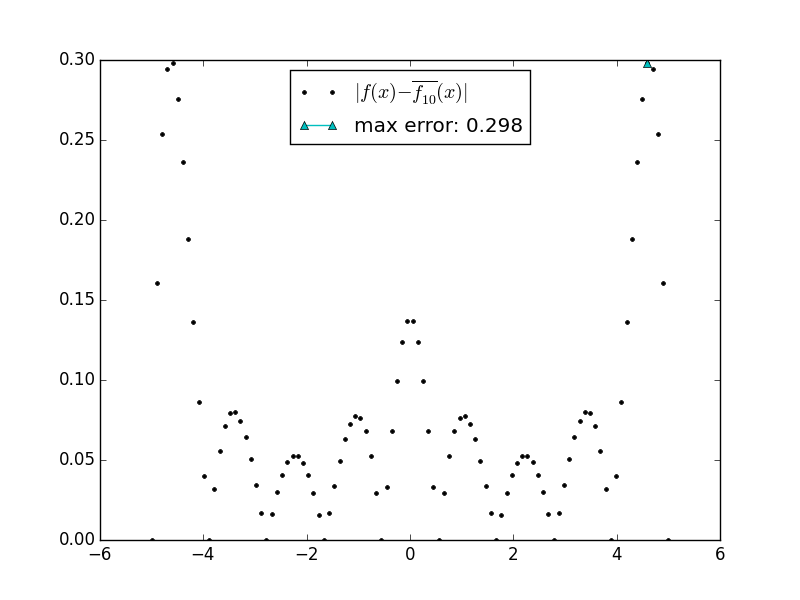
\includegraphics[scale=0.65]{figures/problem4_e_010points.png}}\\
The following graphs show $f(x)$ and its polynomial approximation $\overline{f_{20}}(x)$ for 20 equally spaced points, along with the error of the approximation.\\
\centerline{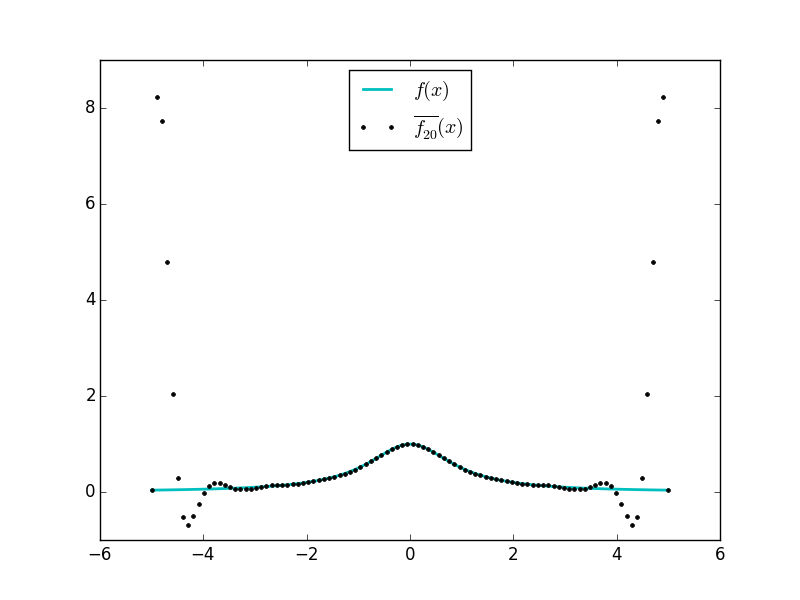
\includegraphics[scale=0.65]{figures/problem4_d_020points.png}}\\
\centerline{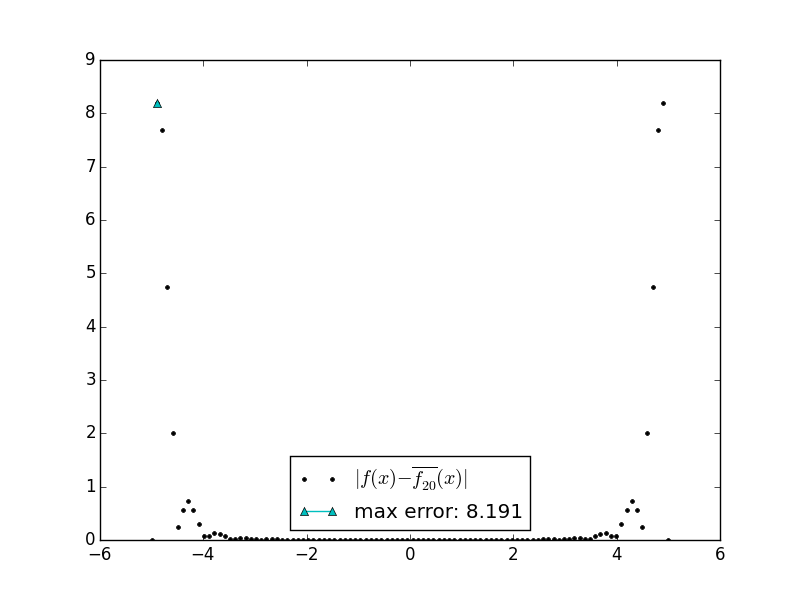
\includegraphics[scale=0.65]{figures/problem4_e_020points.png}}\\
The following graphs show $f(x)$ and its polynomial approximation $\overline{f_{30}}(x)$ for 30 equally spaced points, along with the error of the approximation.\\
\centerline{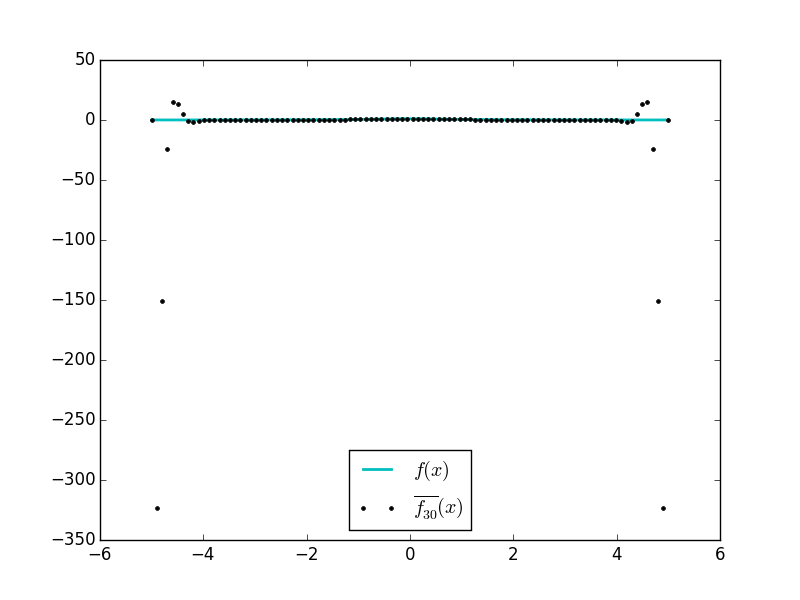
\includegraphics[scale=0.65]{figures/problem4_d_030points.png}}\\
\centerline{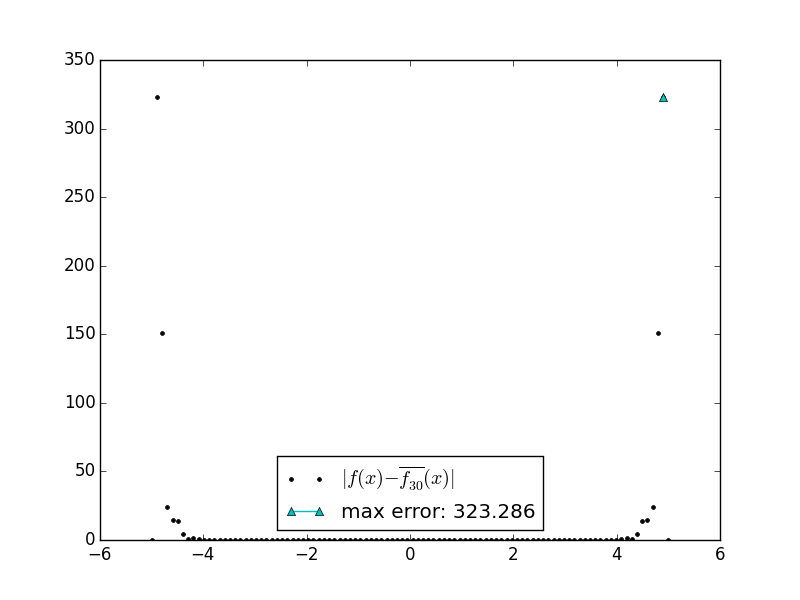
\includegraphics[scale=0.65]{figures/problem4_e_030points.png}}\\
The divided difference table for $n=5$, printed in lines 9 and 10 from the code above, is given below.
\begin{verbatim}
[[-5.          0.03846154  0.0397878   0.06100796 -0.0265252   0.00530504]
 [-2.5         0.13793103  0.34482759 -0.13793103  0.0265252   0.        ]
 [ 0.          1.         -0.34482759  0.06100796  0.          0.        ]
 [ 2.5         0.13793103 -0.0397878   0.          0.          0.        ]
 [ 5.          0.03846154  0.          0.          0.          0.        ]]
\end{verbatim}
For clarity, below is a nicely-formatted \LaTeX \ table.
\begin{table}[H]
    \centering
    \begin{tabular}{||l|l|l|l|l|l||}\hline\hline
    $x_i$ & $f[x_i]$ & $f[x_i, x_{i+1}]$ & $f[x_i, x_{i+1}, x_{i+2}]$ & $f[x_1, \dots, x_{i+3}]$ & $f[x_i, \dots, x_{i+4}]$ \\\hline\hline
$-5.$ & $0.03846154$ & $0.0397878$ & $0.06100796$ & $-0.0265252$ & $0.00530504$ \\\hline
$-2.5$ & $0.13793103$ & $0.34482759$ & $-0.13793103$ & $0.0265252$ & $0.$ \\\hline
$0.$ & $1.$ & $-0.34482759$ & $0.06100796$ & $0.$ & $0.$ \\\hline
$2.5$ & $0.13793103$ & $-0.0397878$ & $0.$ & $0.$ & $0.$ \\\hline
$5.$ & $0.03846154$ & $0.$ & $0.$ & $0.$ & $0.$ \\\hline\hline
    \end{tabular}
\end{table}
\noindent As shown in the error plots above, the maximum error does not decrease as the number of points increases.  In fact, quite the opposite is true.
\begin{table}[H]
    \centering
    \begin{tabular}{||c|c||}\hline\hline
    & {\bf Maximum value} \\
    {\bf Function} & {\bf on $[-5, 5]$} \\\hline\hline
    $|f_{05}(x) - \overline{f_{05}}(x)|$ & $0.438$ \\\hline
    $|f_{10}(x) - \overline{f_{10}}(x)|$ & $0.298$ \\\hline
    $|f_{20}(x) - \overline{f_{20}}(x)|$ & $8.191$ \\\hline
    $|f_{30}(x) - \overline{f_{30}}(x)|$ & $323.286$ \\\hline\hline        
    \end{tabular}
\end{table}
\noindent This seems like a contradiction to the Weierstrass Theorem, which states that any function continuous on a closed interval can be uniformly approximated within any prescribed tolerance by some polynomial.  However, it is {\it not} a contradiction.  Having found some polynomials that do not adequately approximate $f(x)$ near the endpoints of the interval does not prove that there is no such function that does.  It may be the case that we have chosen our data points poorly.  It may be that equally-spaced data points for the entire interval is not the best way to approximate $f(x)$.  As an experiment, let us choose 20 equally-spaced points in $[-5.0, -3.15]$, 11 equally-space points in $[-3.0, 3.0]$, and 20 equally-spaced points in $[3.15, 5.0]$.  This way our set of points is more dense toward the edges of the interval $[-5.0, 5.0]$, and less dense where the function peaks (at $x = 0$).  I used the following code to produce my NumPy array and graph my approximation and the error plot:
\begin{lstlisting}[language=Python, caption=Attempting Different Data Sets for Better Approximations]
intvl_1 = np.linspace(-5.0, -3.15, 20)
intvl_2 = np.linspace(-3.0, 3.0, 11)
intvl_3 = np.linspace(3.15, 5.0, 20)
first_append = np.append(intvl_1, intvl_2)
x_try = np.append(first_append, intvl_3)

DD_try = DivDiffs(x_try, runge)
interp_try = makePolynomial(DD_try)

x_100     = np.linspace(-5.0, 5.0, 100)
error_100 = abs(runge(x_100) - interp_try(x_100))
max_y     = max(error_100)
max_index = list(error_100).index(max_y)
max_x     = list(x_100)[max_index]

runge_label        = "f(x)"
runge_interp_label = "\overline{f_{%.02d}}(x)" % 51
runge_error_label  = "|%s - %s|" % (runge_label, runge_interp_label)

file_name = "figures/problem4_g_50points.png"
plt.figure()
plt.plot(x_100, runge(x_100), "c", linewidth = 2., label = r"$%s$" % runge_label)
plt.plot(x_100, interp_try(x_100), ".k", label = r"$%s$" % runge_interp_label)
plt.legend(loc=0)
plt.savefig("%s/%s" % (DIRECTORY, file_name), format = 'png')
plt.close()

file_name = "figures/problem4_g_error_50points.png"
plt.figure()
plt.plot(x_100, error_100, ".k", label = r"$%s$" % runge_error_label)
plt.plot(max_x, max_y, c="c", marker="^", label = "max error: %.05f" % max_y)
plt.ylim(0, 0.0018)
plt.legend(loc=0)
plt.savefig("%s/%s" % (DIRECTORY, file_name), format = 'png')
plt.close()
\end{lstlisting}
\noindent The following graphs show $f(x)$ and its polynomial approximation $\overline{f_{51}}(x)$ for 51 data points (not equally-spaced), along with the error of the approximation.\\
\centerline{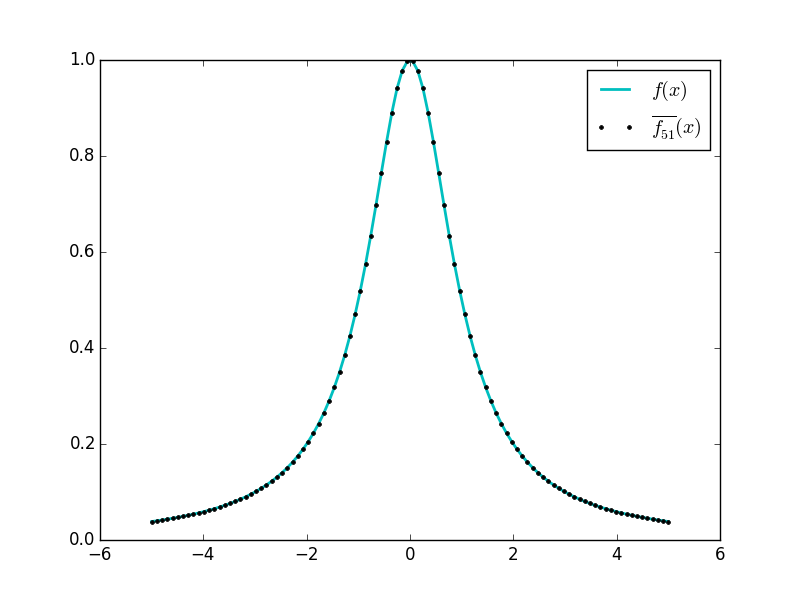
\includegraphics[scale=0.65]{figures/problem4_g_51points.png}}\\
\centerline{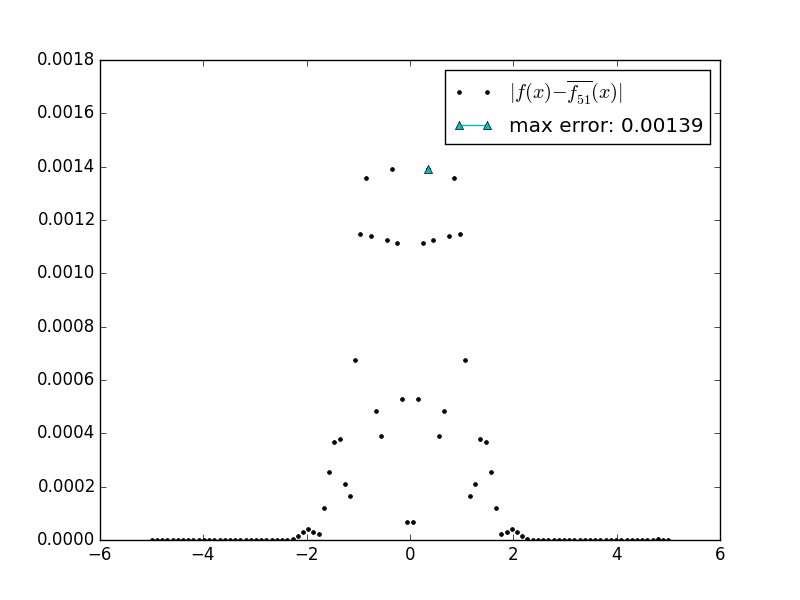
\includegraphics[scale=0.65]{figures/problem4_g_error_51points.png}}\\
Clearly, it is possible to obtain better approximations with many points, but the points must be chosen wisely.  In this case, $f(x)$ was better approximated when the data points were more dense on the edges of the interval.

%\pagebreak
%\begin{thebibliography}{99}
%
%\bibitem{Abrams1997b}
%Abrams, P.~A. and Matsuda, H.
%Prey Adaptation as a Cause of Predator-Prey Cycles.
%\emph{Evolution}
%1997, 51:1742-1750.
%
%\bibitem{Chavez2001}
%Brauer, F., Castillo-Chavez, C.
%Mathematical Models in Population Biology and Epidemiology.
%Springer,
%2011. Print.
%
%\bibitem{Boyce2012}
%Boyce, W. E., and DiPrima, R. C.
%Elementary Differential Equations and Boundary Value Problems %10\textsuperscript{th} ed.
%Wiley Global Education
%2012. Print.
%
%\bibitem{Saloniemi1993}
%Saloniemi, I.
%A Coevolutionary Predator-Prey Model with Quantitative Characters.
%\emph{American Naturalist}
%1993, 141:880-896.
%
%\bibitem{Schreiber2011}
%Schreiber, S.~J., B$\ddot{\mbox{u}}$rger,  R., and Bolnick,  D.~I.
%The Community Effects of Phenotypic and Genetic Variation within a Predator %Population.
%\emph{Ecology}
%2011,  92(8):526-543. 
%
%\end{thebibliography}

\end{document}